\subsection{Discussion}
\label{cic:sec:discussion}




Our survey and interview results (\Cref{cic:sec:Results-all}) show that smart home owners \emph{navigate across} layers of proxy-based control, from central, i.e., several proxies, to physical control, i.e., zero proxies. %\igc{and device-based control? (does proxy spectrum INCLUDE device control? again, an issue with definitions being unclear; in any case, reiterate here what yo umean)} 
as they orchestrate intent, and that the spectrum of smart device control plays a major role in user preferences and experiences, echoing the intuition by \citet{davidoff2006principles, brush2011home} that homes should support everyday experiences rather than mere device operation. We connect these findings to HCI and ubiquitous computing by reframing control as \emph{transition} along two spectra (\Cref{cic:fig:dual-spectrum}): (1) the %\igc{emphasize these phrases (names for the 2 spectra)} 
\emph{locus of execution} (from centralized to local), which reflects where a device action might be initiated from, whether through a hub or on the physical device,
and (2) the \emph{exposure of the system} (from seamless to seamful),  i.e., how users perceive device control, from having to set-and-forget to having fine-grained control of the devices% \igc{that is too long a sentence (for (2))}
. This {\it dual-spectrum} view helps explain %when \igc{
under what conditions %? (when is too vague, and appears to refer to time)}
people keep infrastructures invisible and when they purposefully reveal seams, and it grounds actionable implications for hubs, vendor apps, and household governance.  %\igc{this is too  abstract a way of writing. We used to have a figure here showing the two orthogonal spectra, right? Anything to make the writing less abstract would help.}

These spectra are orthogonal: a person can operate centrally and hide seams for low-stakes routines, then shift downstream and reveal seams to accomplish a fine-grained adjustment that the hub cannot reach (e.g., voice can stream a camera feed, but pan, tilt, and zoom (PTZ) requires the vendor app). Our participants' perspectives revealed the importance of designing for these transitions, rather than a single point. We expand on this below, with examples.

\subsubsection{From device control to orchestrating transitions}
\label{cic:sec:dualControl}

In the consumer landscape, platform marketing emphasizes \emph{seamlessness} and \emph{invisible} infrastructure; for example, Matter aims to make multi-brand integration routine, promising an architecture that ``just works'' in daily use~\cite{matter}. Users move freely along the spectrum, guided by
situational factors such as perceived convenience, perceived reliability, and task.

While these narratives shape expectations,~\citet{bell2007yesterday} argue that the seamless vision of ubiquitous computing remains less of a lived reality. In HCI, seamful design argues that exposing implementation gaps can be useful for diagnosis and adaptation~\cite{chalmers2003seamful, chalmersSeamfulDesignShowing2003}, while infrastructure studies remind us that infrastructures are ordinarily taken for granted and become visible at breakdown, adoption, or scaling~\cite{star1994infra}. Managing and constructing a smart home space requires users to constantly weigh tradeoffs between convenience and control, automation and transparency, and speed and flexibility as discussed in~\Cref{cic:sec:relatedWorks-smarthome}.

We mapped participants' interaction journey between physical and central control onto two orthogonal spectra that distinguished \emph{where} individuals are operating and controlling their devices from, and \emph{how} people are handling rough edges%
%\igc{sentence seems  ungrammatical-pls check (I think two "are"s are needed.}
.

% \igc{Make these para headers textbf-textit rather than paragraph, to make them pop.}
\noindent\textbf{The locus of execution spectrum: Proxy-based control $\leftrightarrow$ Physical control.}
The \emph{locus of execution} refers to the level of abstraction at which smart home users control their devices~\cite{perrault2015physical, rip2002identifying}: whether controlling them through a hub/ecosystem (central; shared scenes, routines, voice assistants) or invoking actions through the device-specific app (local; vendor app, on-device UI, physical interface). Higher-level proxy-based loci tend to provide \emph{breadth} across devices and people; local loci provide \emph{depth and assurance} via device-specific features, histories/logs, firmware access, and tangible fallbacks~\cite{chen2025expressing, corno2021users}. 

Movement across loci is common. In our data, shifts toward physical control were precipitated by capability ceilings at the hub, device-specific needs (e.g., camera PTZ control or schedule histories), governance constraints (account scoping, co-editing), and lifecycle events (router/ISP swaps, device replacement). For instance, participants with larger installations described relying on a hub for routine scenes yet still opening brand apps to adjust advanced parameters or to locate firmware updates (\Cref{cic:subsec:tradeoffs}). These participants treated proxy-based control as a default broadcast channel for tasks, but reserved physical or local controls as authoritative sources about specific device states or capabilities.

\noindent\textbf{The seam practice spectrum: Seam hiding $\leftrightarrow$ Seam revealing.}
In an infrastructure such as a smart home, \textit{seams} are the imperfections and complexities of systems~\cite{madakam2014smart}. While the locus of execution spectrum captures \emph{where} users act in the infrastructure, the seam practice spectrum captures \emph{how} they choose to manage the visibility of that infrastructure as they move across layers. Rather than treating seams as a fixed property of the system, our data show seam practice as an ongoing, situated accomplishment: participants actively decide when to keep control flows invisible and when to expose the underlying infrastructure to get leverage. This everyday seam hiding or seamlessness reduces cognitive and social overhead (e.g., making it easier for other household members to just talk to the assistant rather than learning multiple apps), and resonates with prior critiques of frictionless interfaces~\cite{hengesbach2022undoing,inman2019beautiful}.

When smart device expectations failed, participants engaged in deliberate seam revealing processes that went beyond what prior seamful design examples~\cite{kuznetsov2012seams,chalmers2004social}. Participants systematically peeled back layers. They start at a high-level proxy (hub or voice), then open vendor apps to inspect device states, history, or logs, and finally manipulate device-local controls or power to test hypotheses about what was failing (\Cref{cic:fig:survey-troubleshooting-sequence}). By \emph{appropriating} seams as diagnostic handles, validating prior work describing how technical exposures serve as resources for sensemaking during breakdown~\cite{dao2021bad, benford2006can}. Our dual-spectrum lens (\Cref{cic:fig:dual-spectrum}) frames~\textbf{seam hiding as the default when proxy-based locus of execution is stable, whereas seam revealing is a manual intervention for users to regain precision, understanding, or accountability when that locus fails them.}

%\del{\emph{Seam practice} refers to \emph{how} rough edges are handled: when things ``just works,'' controls and flows were kept invisible to provide a seamless experience~\cite{hengesbach2022undoing,kuznetsov2012seams,inman2019beautiful,chalmers2004social}.  On the other hand, purposefully exposed control exposed options for users to diagnose or act (opening native panels or logs, re-pairing/renaming, flipping physical toggles). Hiding seams reduces overhead in routine operation; revealing seams restores precision, understanding, and control during uncertainty or failure. In our data, moves along this axis were driven by recognition ambiguity, interoperability gaps, network/power issues, privacy or assurance needs, and multi-user coordination and auditability (\Cref{cic:subsec:controlspectrum} and \Cref{cic:subsec:tradeoffs}).~\Cref{cic:fig:survey-troubleshooting-sequence} illustrates how participants hid seams during routine use, then revealed seams to diagnose and act when features were fragmented or missing (e.g., one interviewee noted that voice could stream a camera feed but could not actuate PTZ, prompting a switch to the native app).}


% \igc{weird para header in bold inconsistent with previous para header formats}
\noindent\textbf{Transitions as design.} By creating this dual spectrum, we notice that movement across control layers should be preserved rather than eliminated; this gives individuals agency to trade off convenience against fine-grained control, accountability, and recovery. Rather than arguing the control scheme for ``hub vs.\ per-brand'' claims, the agency for participants to move across the spectrum is a less explored design space where participants adopted \emph{central\,+\,invisible} configurations for repetitive, low-stakes tasks; they shifted toward \emph{physical\,+\,seamful} configurations for fine-grained control, accountability, or assurance. This perspective also addresses timeliness critiques: even as standards evolve, households will continue to encounter breakdowns, maintenance, mixed accounts, and perceived risk---conditions that \emph{require} traversing axes.

\begin{figure}[t!]
    \centering
    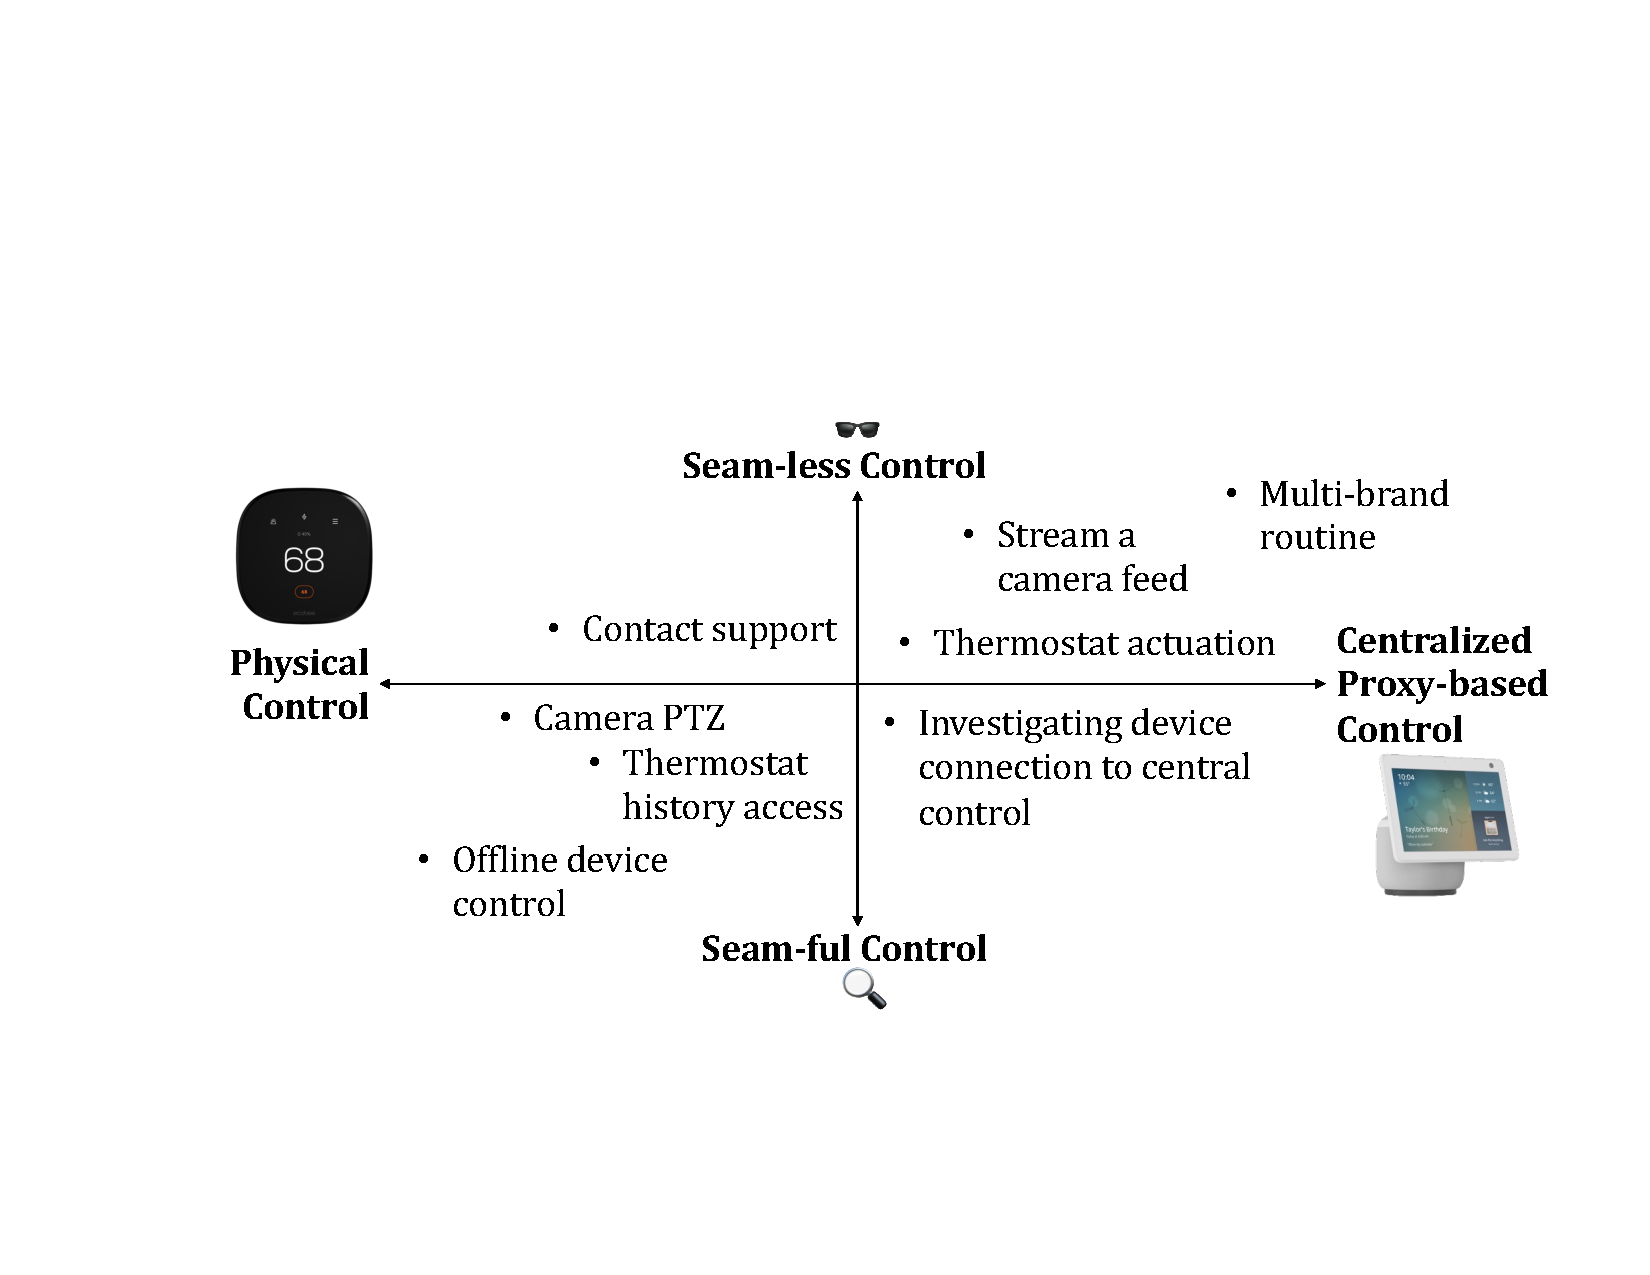
\includegraphics[width=0.7\linewidth,alt={Two-dimensional quadrant diagram. The horizontal axis runs from physical control on the left to proxy-based control on the right; the vertical axis runs from seam-ful at the bottom to seam-less at the top. Top-right (proxy-based, seam-less): streaming a camera feed and thermostat actuation. Bottom-right (proxy-based, seam-ful): investigating a device's connection to central control. Bottom-left (physical, seam-ful): camera pan-tilt-zoom (PTZ), thermostat history access, offline device control. Top-left (physical, seam-less): contacting support. Users can navigate the locus axis freely, but vendors give only limited navigability of the seam axis.}]{ControlInContext/figures/Dual smart home control spectrum-expanded.pdf}
    \caption{Dual smart home control spectrum. The proxy-based vs physical control axis refers to the locus of execution spectrum, whereas the seam-less vs seam-ful axis refers to the seam practice spectrum. The user can navigate the locus spectrum based on their needs, whereas the vendors give limited navigability of the seam spectrum, almost enforcing how users will experience their control interfaces' integration.}
    % \Description{
    % Two-dimensional quadrant diagram with perpendicular axes. 
    % The horizontal axis runs from physical control on the left to proxy-based control on the right. 
    % The vertical axis runs from seam revealing at the bottom to seam hiding at the top. 
    % In the top-right quadrant, proxy-based control plus seam hiding, examples are streaming a camera feed and thermostat actuation. 
    % In the bottom-right quadrant, proxy-based control plus seam revealing, the example is investigating device connection to central control. 
    % In the bottom-left quadrant, physical control plus seam revealing, examples include camera pan-tilt-zoom, thermostat history access, and offline device control. 
    % In the top-left quadrant, physical control plus seam hiding, the example is contacting support.
    % }
    \label{cic:fig:dual-spectrum}
\end{figure}

\subsubsection{Smart homes as information ecologies of control}
Our work reveals that when a user considers adding or modifying devices in their home, or even interacting with their home, it is not just the devices, but the modes of control that matter. The IoT/smart home device marketplace typically frames value in terms of devices with ``more'' or ``smarter'' features~\cite{sun2024unfulfilled, basarir2022identifying, nasirinejad2023evaluating}. However, our findings show that the ways those devices can be controlled are equally important for how people evaluate and live with smart home devices over time. 
%
Put more technically, smart homes are often described as a single coherent system~\cite{yar2021towards, domb2019smart, cicirelli2016design}; however, our findings suggest a different framing, where smart homes are thought of as information ecologies of control. While traditional information ecology theory focuses broadly on human-technology configurations~\cite{lyle2020s, mcnely2010exploring}, participant experiences show that the loci of execution also function as a significant part of this ecology. Households cultivate combinations of these ``species,'' or groups of devices and associated control modalities (such as P5, who had different loci depending on the room of their house), and adjust them as their setup, routine, and environment change. 
%\igc{seems a bit thin. Perhaps add a ref to another of our users in the user study? (just one user could be an outlier)}

Movements along the locus of execution spectrum are less about isolated interface preferences and more about ecological preference. Adding a new device, changing homes or internet providers, experiencing repeated failures, or other external stimuli prompted participants to re-balance their control ecology. This included disabling a routine (P3), abandoning a hub/device (P5), or falling back to physical device control (P8). Furthermore, troubleshooting was revealed as a moment where not only a malfunctioning device was examined, but the entire smart home ecology. 

Participants continuously evaluated their smart home ecology in terms of its usefulness and ability to integrate into their day-to-day lives. This evaluation helped participants identify which loci of execution they were willing to depend on. By framing smart homes as evolving information ecologies, which include loci of execution, we shift attention from evaluating individual products to understanding how they participate in and reshape household ecologies. Next, we translate this lens into concrete design implications and open questions for future smart home systems. 

\subsubsection{Design implications and open questions}
\label{cic:sec:implications_future}
A dual-spectrum stance shifts attention from choosing a ``best'' locus to \emph{supporting transitions} to making crossings legible, low-friction, and accountable. 
Importantly, \emph{control loci do not map one-to-one to physical devices}: the hardware could contain several loci (third-party app vs.\ second-party app vs. first-party physical control), and a routine state can be ``hidden'' while device state remains visible or vice versa.

\noindent\textbf{Design hubs for transparency and ceilings.}
Centralized interfaces should disclose \emph{capability ceilings} and provide explicit~\emph{bridges} to device-local depth. When a hub cannot reach feature/parameter-level control (e.g., camera PTZ, thermostat histories~\cite{stopps2021anyone}), the UI should indicate this and provide a deep-link to the native panel. 
This reduces ``hunt-the-setting'' failures, lessens the mental burden of switching platforms and remembering device names, and matches observed escalations in \Cref{cic:subsec:tradeoffs}. Designing away these transitions in pursuit of a perfectly seamless hub risks trapping users at a single, brittle locus of execution with no graceful way to regain control when expectations are violated.

%igc{Side comment: this is really useful. Often today HVAC technicians (including mine) routinely recommend AGAINST installing NEST thermostats because they tell me, "It won't give you as much power as the native TRANE thermostat." (and I can never know for sure if that is true, without actually installing and using it)}

\noindent\textbf{Provenance and interoperability legibility.}
When scenes (predefined multi-device routines) span mixed brands or partial standards support, displaying a pre-flight check with the ``weakest link'' highlighted and present guided degradation paths (e.g., ``device offline---try local control''), along with \emph{who executed what, where}. Provenance-forward feedback increases trust when hub-instantiated actions trigger device responses, helping smart home users construct mental models and accelerating troubleshooting paths we observed in \Cref{cic:subsec:navigatingcontrol}. This approach prioritizes coverage over device-specific depth. This works well for routine, low-stakes state changes and whole-home coordination; when a capability ceiling or failure is detected, the pre-flight/provenance cues a \emph{depth-first} pivot (e.g., open vendor app, use a physical control) to resolve the outlier. For example, centralized interfaces should be honest about what they cannot accomplish and point users to the right vendor/device-specific path when they hit those limits.

\noindent\textbf{Governing households while respecting privacy.}
Proxy-based interfaces should treat routines and devices as shared resources with roles, co-editing, and change histories by default (\Cref{cic:tab:confusion}). Revealing device states and last-known state offers tangible backstops for high-stakes actions, helping smart home users navigate across the two spectra. For example, prior HCI work shows users prefer simple, proactive controls in the home and benefit from tangible mechanisms for privacy and assurance~\cite{windl2025privacyhub,abdi2021privacy, de2015homerules}. This design echoes the delicate balance wherein tangible interfaces reveal how household members shift between central and local loci and between hiding and revealing seams. In practice, this requires deeper engagement with stakeholders in the smart home, especially those whose voices are traditionally unheard (children, secondary users, nannies, etc.), as current spectra navigating designs often hurt these users most~\cite{10.1145/3544548.3581504, 10.1145/3613904.3641962}. Working with such users and including them as an integral part of the design process helps establish both smart home devices and their corresponding control spectra as ``sources of empowerment'', which can make moving between control methods in the home a less daunting experience~\cite{10.1145/3613904.3642866}.

\noindent\textbf{Open Questions: Evaluating Transition Quality.}
Our work opens up two further directions on transition quality. First, there is a need to characterize what information and granularity different user roles (and levels of expertise) need at the moment of crossing to be effective without overload. Second, there is a need to develop evaluation metrics for transition quality: e.g., time to successful handoff; rate of stranded actions; clarity of ceilings and provenance; and recovery burden after lifecycle events (\Cref{cic:subsec:controlspectrum}).
